\documentclass[11pt,a4paper]{article}

\usepackage[margin=1in]{geometry}
\usepackage{amsmath}
\usepackage{amssymb}
\usepackage{graphicx}
\usepackage{booktabs}
\usepackage{natbib}
\usepackage[hidelinks]{hyperref}
\usepackage{xcolor}

% Arcminute symbol — not defined in base LaTeX.
\providecommand{\arcmin}{^{\prime}}
% Textual Lambda-CDM for PDF outlines/bookmarks so hyperref does not warn.
\providecommand{\LambdaCDM}{\texorpdfstring{$\Lambda$CDM}{LambdaCDM}}

\title{An interpretable, trials-corrected machine-learning search for Penrose Hawking points in the Planck 2018 cosmic microwave background}

\author{Ram Chand \\
Department of Natural Sciences \\
The Begum Nusrat Bhutto Women University, Sukkur, Sindh, Pakistan \\
\texttt{ram.chand2k11@yahoo.com}}

\date{\today}

\begin{document}

\maketitle

\begin{abstract}
\noindent \textbf{Context.} Roger Penrose's conformal cyclic cosmology (CCC) predicts that supermassive black holes evaporating during the previous cosmic aeon leave small, quasi-circular temperature imprints on the cosmic microwave background (CMB) of the current aeon --- ``Hawking points'' --- of order one degree in angular size and tens of microkelvin in central amplitude \citep{penrose_ccc_2010,an_amnp_2018}. The original ring-variance search of \citet{gp_2010a,gp_2010b} and the Gaussian-template search of \citet{an_amnp_2018} reported candidate detections, but \citet{jow_scott_2020} showed the significances dissolve into the Gaussian $\Lambda$CDM null under a proper look-elsewhere correction.

\noindent \textbf{Aims.} We identify three co-occurring limitations of the existing Hawking-point search literature --- template dependence, the absence of an inspectable decision rule, and inadequate trials-factor calibration --- and build a search pipeline that addresses all three simultaneously. We apply it to the four Planck 2018 component-separation CMB maps and report the significance of every candidate signal.

\noindent \textbf{Methods.} For each candidate sky patch we compute a 40-dimensional vector of physically-named features: a ring-variance profile in the sense of \citet{gp_2010a}, spherical wavelet coefficients \citep{vielva_2004}, Minkowski functionals of local excursion sets \citep{schmalzing_gorski_1998}, and local moments. A whitened multivariate Gaussian density model trained on 1000 Gaussian $\Lambda$CDM null simulations assigns an anomaly score. We reduce this score to a compact linear combination of the input features by ridge regression (``symbolic distillation''), and calibrate its significance against the empirical distribution of the sky-wide maximum of the compact statistic across the null ensemble. The trials factor is absorbed by construction \citep{gross_vitells_2010}. Candidates are further required to appear consistently in all four Planck component-separation maps and to pass a robust extreme-pixel scrub.

\noindent \textbf{Results.} The trials-corrected p-values are uniform on 200 held-out Gaussian control simulations (Kolmogorov--Smirnov $p_{\text{KS}} = 0.48$). The compact statistic recovers the classical Gurzadyan--Penrose ring-variance ratio as one of its dominant terms, and identifies the Minkowski perimeter $V_1$ of $\pm 1\sigma$ excursion sets as a new co-dominant channel. Under the official Planck common confidence mask, no candidate exceeds the trials-corrected $\alpha = 0.01$ threshold in more than one of the four maps except a single cluster at galactic coordinates $(l, b) \approx (133^\circ, -24^\circ)$. Its morphology is asymmetric and does not match the AMNP-2018 template. A Planck 353\,GHz thermal-dust cross-check finds the candidate direction is 0.57 times the median dust brightness and 0.49 times the median dust variability of same-galactic-latitude controls, ruling out a shared foreground residual.

\noindent \textbf{Conclusions.} We report a calibrated non-detection of AMNP-2018-shape Hawking points above about $80\,\mu\mathrm{K}$ at $\sim 1^\circ$ angular scale in Planck PR3 data. The physical origin of the $(l, b) \approx (133^\circ, -24^\circ)$ cluster is unresolved between a rare Gaussian $\Lambda$CDM null-tail configuration and a genuinely anomalous CMB feature; higher-$N$ calibration is required to distinguish these. All code and analysis products are publicly available at \url{https://github.com/ramc77/CCC-HawkingPoints}.

\smallskip
\noindent\textbf{Key words.} cosmic microwave background --- cosmology: observations --- cosmology: theory --- methods: statistical --- methods: data analysis
\end{abstract}

\section{Introduction}\label{sec:intro}

The cosmic microwave background (CMB) records the state of the universe at the epoch of last scattering, some 380{,}000 years after the Big Bang. To the precision of current instruments, the CMB temperature fluctuations are statistically isotropic and consistent with the near-Gaussian random field predicted by inflationary $\Lambda$CDM cosmology \citep{planck2018_i,planck2018_vi}. Any alternative to inflation must reproduce these statistics, or must predict a distinguishable deviation that has escaped detection.

\subsection{The Hawking-point prediction of CCC}\label{sec:ccc}

Roger Penrose's conformal cyclic cosmology (CCC) is one such alternative \citep{penrose_ccc_2010}. In CCC the universe passes through an infinite sequence of aeons. Each aeon begins at a smooth, matter-free conformal boundary that plays the role of a Big Bang, and this boundary is not vacuum in the ordinary sense: it is the conformally rescaled future infinity of the preceding aeon, into which the fields of the previous aeon have been extended. Physical scales at the beginning of one aeon are related to physical scales at the end of the previous one by a Weyl rescaling of the metric, and energy carried by massless quanta survives the transition.

Supermassive black holes that evaporate via Hawking radiation \citep{hawking_1975} late in an aeon are the largest single sources of massless radiation in that aeon. Their evaporation signal passes into the next aeon and, in the CMB of the current aeon, appears as small circular temperature excesses. \citet{an_amnp_2018} refer to these excesses as ``Hawking points''. The prediction is quantitative: the features should have angular sizes of order $1^\circ$ (set by the horizon size at last scattering divided by the redshift-integrated conformal distance to the CMB), and central amplitudes of order tens of microkelvin (a few times the $\sigma \simeq 50\,\mu\mathrm{K}$ CMB fluctuation amplitude at that angular scale). Their sky positions are unpredicted, since they reflect the random locations of the parent black holes in the previous aeon.

\subsection{Prior searches and the look-elsewhere effect}\label{sec:prior}

Testing the Hawking-point prediction is a search problem: given the observed CMB temperature map, do any small regions show a temperature morphology inconsistent with the Gaussian $\Lambda$CDM null? Three attempts and one influential re-analysis have appeared in the literature.

\citet{gp_2010a,gp_2010b} reported low-variance concentric circles in \emph{Wilkinson Microwave Anisotropy Probe} (\emph{WMAP}) data. They defined a ring-variance statistic, the variance of temperature in a narrow inner annulus divided by the mean variance in a set of outer annuli. This statistic is small in any direction where the CMB happens to be unusually quiet on the corresponding angular scale. They evaluated the statistic at every candidate center on the sky, then compared its sky-wide maximum against approximately one thousand Gaussian $\Lambda$CDM simulations, and reported a significant excess.

\citet{an_amnp_2018} refined the analysis with a specifically Hawking-point ansatz. Rather than a ring statistic they fit a Gaussian radial temperature profile of $\sim 1^\circ$ opening angle to Planck component-separation maps, and reported candidate detections at central amplitudes of a few tens of microkelvin.

\citet{jow_scott_2020} then revisited both claims using a Bayesian model comparison that folded in the look-elsewhere effect \citep{gross_vitells_2010}. The look-elsewhere effect is the multiple-comparisons penalty that any all-sky search must pay: the number of statistically independent patches at $\sim 1^\circ$ scale on the full sky is of order $10^4$, so a per-patch p-value of $10^{-3}$ is expected to occur about ten times in a truly Gaussian $\Lambda$CDM sky by chance alone. Quoting the smallest per-patch p-value as if it were the global significance overstates the evidence by a factor equal to the number of trials. When \citet{jow_scott_2020} performed the joint calculation, the earlier Hawking-point anomalies were consistent with the Gaussian $\Lambda$CDM null at posterior-odds unity.

The methodological lesson generalises. Any CMB anomaly claim that quotes a per-patch significance without a trials-corrected joint calibration is unlikely to survive a careful re-analysis. The correct null distribution is not the per-patch statistic; it is the distribution of the sky-wide maximum of that statistic across a large ensemble of Gaussian $\Lambda$CDM realizations. The correct question that any significance answers is ``how surprising is this excess \emph{anywhere} on the sky?''.

\subsection{The one machine-learning attempt to date}\label{sec:bodnia_review}

The one machine-learning search in the literature is HawkingNet \citep{bodnia_2022}, a supervised residual convolutional-neural-network classifier trained on synthetic AMNP-shape Hawking-point templates embedded in real Planck and \emph{WMAP} data. On the real data the classifier reported candidate excesses, but the excesses were driven by a small number of extreme individual pixels: single cosmic-ray hits and calibration outliers that survived component separation. Once those outlier pixels were masked, no significant detection remained.

Two methodological lessons follow. First, individual outlier pixels can counterfeit whole families of circular anomalies through their effect on low-order variance statistics; any pipeline must include an explicit extreme-pixel check. Second, a supervised classifier trained on one specific template shape has no sensitivity to a signal of a different shape, and its decisions cannot be inspected physically or compared to classical statistics.

\subsection{Research gap and contribution of this paper}\label{sec:gap}

The existing Hawking-point search literature suffers from three co-occurring methodological limitations. Any one of them is enough to make a claim of detection unreliable; taken together they explain why the field has oscillated between claims and refutations for more than a decade.

\begin{enumerate}
\item[\textbf{L1. Template dependence.}] Every published search --- ring-variance in \citet{gp_2010a,gp_2010b}, Gaussian radial template in \citet{an_amnp_2018}, and supervised deep-learning template in \citet{bodnia_2022} --- assumes a specific circular signal shape. A signal that departs from this shape (for instance, an asymmetric or off-center feature) is missed by construction.
\item[\textbf{L2. Inspectability void.}] The one machine-learning search to date is a supervised black-box classifier. Its decisions cannot be checked against physical intuition or compared to classical statistics. When it reports a candidate, one cannot tell from the classifier alone whether the candidate resembles a Hawking point or an outlier pixel; the diagnostic of \citet{bodnia_2022} was made after the fact.
\item[\textbf{L3. Trials-factor calibration.}] The earlier searches did not fold in the look-elsewhere effect at the level of the calibration null distribution; \citet{jow_scott_2020} added it post hoc. A pipeline whose calibration null is not, from the beginning, the distribution of the sky-wide maximum of the search statistic is at risk of the Jow--Scott failure mode.
\end{enumerate}

The pipeline described in this paper addresses all three limitations simultaneously. In outline:
\begin{itemize}
\item[(i)] To defeat \textbf{L1}, we do not assume any Hawking-point template. We learn the distribution of Gaussian $\Lambda$CDM CMB skies directly from 1000 null simulations, and score any real patch by how unlike that null it looks.
\item[(ii)] To defeat \textbf{L2}, we compress the learned anomaly score into a compact linear combination of physically-named CMB features (ring-variance profile, spherical wavelet coefficients, Minkowski excursion-set functionals, local moments), so that the machine's decision is inspectable and directly comparable to the classical Gurzadyan--Penrose ring-variance statistic.
\item[(iii)] To defeat \textbf{L3}, we calibrate the statistical significance against the empirical CDF of the sky-wide maximum of the compact statistic across the null ensemble. This absorbs the look-elsewhere effect by construction, and we verify calibration by requiring uniform p-values on 200 independent Gaussian control simulations.
\item[(iv)] We further require every claimed above-threshold candidate to appear consistently across the four Planck 2018 component-separation maps, and to survive an extreme-pixel scrub in which we mask pixels whose $|T - \operatorname{median}|$ exceeds three times the median absolute deviation of the disc.
\end{itemize}

The pipeline is applied to the four Planck 2018 component-separation CMB maps under the official Planck common confidence mask, and we characterise every candidate whose distilled score exceeds the $\alpha = 0.01$ trials-corrected threshold.

Section~\ref{sec:data} describes the data and the null simulations. Section~\ref{sec:method} describes the pipeline in six operational stages. Section~\ref{sec:results} reports the calibration certification (Fig.~\ref{fig:kshist}), the sensitivity floor (Fig.~\ref{fig:sensitivity} and Tab.~\ref{tab:sensitivity}), the distilled anomaly statistic, the cross-pipeline candidate matrix (Tabs.~\ref{tab:consistent_subthresh}, \ref{tab:consistent_supthresh}, \ref{tab:commander_residuals}), and the physical characterisation of the single above-threshold cluster (Fig.~\ref{fig:candidate_maps} and Tab.~\ref{tab:dust_check}). Section~\ref{sec:discussion} discusses the null result and the open interpretation of the above-threshold cluster. Section~\ref{sec:conclusion} concludes.

\section{Data and simulations}\label{sec:data}

\subsection{Planck 2018 component-separation maps}

We use the four Planck PR3 (2018) component-separated CMB temperature maps: SMICA, NILC, SEVEM, and Commander \citep{planck2018_iv}. Each is provided in the Hierarchical Equal-Area isoLatitude Pixelisation (HEALPix) scheme \citep{gorski_2005} at resolution parameter $n_{\text{side}} = 2048$ and with a $5\arcmin$ Gaussian effective beam. All four maps target the same underlying CMB, but they differ in the algorithm used to separate the cosmological signal from galactic foregrounds. SMICA and NILC operate in spherical-harmonic space with different weighting schemes; SEVEM subtracts internal foreground templates; Commander is a Bayesian parametric component fit. Cross-checking a candidate against all four is the strongest single test that a claimed signal is astrophysical rather than an artefact of a particular separation algorithm.

For our search we degrade the maps to $n_{\text{side}} = 512$, corresponding to a pixel scale of about $7\arcmin$. This resolution comfortably resolves the $\sim 1^\circ$ predicted Hawking-point scale and keeps the compute cost of the 1000-simulation null ensemble manageable. We apply the official Planck common confidence mask (\texttt{COM\_Mask\_CMB-common-Mask-Int\_2048\_R3.00}) at the same $n_{\text{side}}$; $62.65\%$ of the sky is retained after masking, with the excluded regions being the galactic plane and known bright compact sources.

\subsection{Gaussian \LambdaCDM{} null ensemble}\label{sec:nullsim}

The pipeline's calibration null is built from $N_{\text{sims}} = 1000$ independent Gaussian $\Lambda$CDM realizations of the CMB temperature sky. The theory temperature angular power spectrum $C_\ell$ is computed with the Code for Anisotropies in the Microwave Background (CAMB, \citealt{lewis_2000}) using fiducial Planck 2018 cosmological parameters \citep{planck2018_vi}: $H_0 = 67.36$\,km\,s$^{-1}$\,Mpc$^{-1}$, $\Omega_b h^2 = 0.02237$, $\Omega_c h^2 = 0.1200$, optical depth $\tau = 0.0544$, and scalar amplitude and tilt $A_s = 2.1 \times 10^{-9}$, $n_s = 0.9649$. Each of the 1000 realizations is drawn from this $C_\ell$ with the HEALPix routine \texttt{synfast} at $n_{\text{side}} = 512$, convolved with a $5\arcmin$ Gaussian beam to match the map resolution, and masked with the same official confidence mask applied to the real data.

We split the 1000 realizations disjointly by simulation identifier, so that training, calibration, and control-check sets are drawn from independent simulations (never from patches of a single simulation, which would share correlated large-scale modes and lead to leakage between splits). The split is: training uses 500 simulations $\times$ 30 patches each = 15{,}000 rows for the density model; calibration uses 300 simulations $\times$ 30 patches each = 9{,}000 rows for constructing the trials-corrected null distribution; and held-out control uses 200 simulations $\times$ 30 patches each = 6{,}000 rows for the Kolmogorov--Smirnov uniformity check.

\section{Method}\label{sec:method}

The pipeline processes each candidate sky patch through six operational stages. In outline: (1) extract a 40-dimensional vector of physically-named features on the patch (Sect.~\ref{sec:features}); (2) score the anomaly of the vector against a density model of the Gaussian $\Lambda$CDM null (Sect.~\ref{sec:density}); (3) measure how the score depends on the amplitude of an injected AMNP-2018 template, giving a detection floor (Sect.~\ref{sec:sensitivity}); (4) build the trials-corrected null distribution of the sky-wide maximum score and verify its calibration (Sect.~\ref{sec:calibration}); (5) reduce the anomaly score to a closed-form linear combination of the input features by ridge regression (Sect.~\ref{sec:distillation}); and (6) require any real-data candidate to appear consistently across the four Planck component-separation maps and to survive a robust extreme-pixel scrub (Sect.~\ref{sec:method_scrub}).

\subsection{Feature extraction on a sky patch}\label{sec:features}

Given a candidate patch center $\hat{n}$ (a unit vector on the sky) and a HEALPix CMB temperature map $T(p)$, the pipeline computes a 40-dimensional feature vector $x(\hat{n}, T)$. Every entry is a physically-named quantity, so the machine's downstream decision can be compared to physical intuition. The features are organised into four families.

\textbf{Radial ring-variance profile (17 features).} Following the Gurzadyan--Penrose construction \citep{gp_2010a}, we choose annular radii $r_0 = 0, r_1, \ldots, r_8 = 2^\circ$ around the patch center. In each of the eight annuli we compute the mean temperature $\mu_k = \langle T \rangle_k$ and the variance $\sigma_k^2 = \operatorname{Var}(T)_k$, giving 16 features. To keep the classical Gurzadyan--Penrose statistic itself in the vector as a labelled dimension, we also record the ratio
\begin{equation}
r_{\text{var}} = \frac{\sigma_{\text{inner}}^2}{\mathrm{mean}_k(\sigma_{\text{outer},k}^2)},
\label{eq:rvar}
\end{equation}
where $\sigma_{\text{inner}}$ is the standard deviation in the innermost annulus and $\sigma_{\text{outer},k}$ is the standard deviation in the $k$-th outer annulus. Small values of $r_{\text{var}}$ correspond to unusually quiet central circles; this is the signature that \citet{gp_2010a} originally sought.

\textbf{Spherical wavelet coefficients (12 features).} A gnomonic projection is a locally flat-sky projection tangent to the sphere at the patch center; distances are undistorted at the projection point and distort by less than one percent across the $5^\circ$ patches we use. We project each patch onto such a plane and apply Mexican-hat wavelets \citep{vielva_2004} at four scales $s \in \{0.25^\circ, 0.5^\circ, 1^\circ, 1.5^\circ\}$. The Mexican-hat wavelet is a bandpass filter of Gaussian-derivative shape, mathematically equivalent to a difference of two Gaussians of matched scales; for each scale we record the mean, variance, and peak absolute value of the wavelet response, giving twelve features. A wavelet whose scale would sit inside less than half a HEALPix resolution element, or would be wider than one third of the patch itself, is set to NaN and filtered before density fitting, as a safeguard against under- or over-sampled scales.

\textbf{Minkowski functionals of local excursion sets (9 features).} The Minkowski functionals \citep{schmalzing_gorski_1998} of a two-dimensional field at threshold $\nu$ are three integral-geometric summaries of the excursion set $E_\nu = \{p : T(p) - \langle T \rangle > \nu \sigma\}$ (the set of pixels whose temperature exceeds the local mean by more than $\nu$ standard deviations). The three functionals are the fractional area $V_0$, the boundary perimeter $V_1$, and the Euler characteristic $V_2$ (the number of connected excursion regions minus the number of enclosed holes). We evaluate them at three thresholds $\nu \in \{-1, 0, +1\}$ and record all nine values.

The standard deviation $\sigma$ used in the excursion definition is critical to the pipeline's robustness. We use the robust median absolute deviation (MAD),
\begin{equation}
\sigma_{\text{MAD}} \;=\; 1.4826 \times \operatorname{median}(|T - \operatorname{median}(T)|),
\label{eq:mad}
\end{equation}
where the constant 1.4826 is the numerical factor that makes $\sigma_{\text{MAD}}$ asymptotically equal to the ordinary standard deviation on data drawn from a Gaussian. Unlike the ordinary standard deviation, $\sigma_{\text{MAD}}$ is not inflated by a small number of extreme pixels. This choice matters directly for the extreme-pixel scrub of Section~\ref{sec:method_scrub}, where a naive $\sigma_{\text{std}}$ would let a bright compact source inflate its own excursion threshold and thereby survive the scrub. We observed this failure mode during pipeline development and fixed it by adopting $\sigma_{\text{MAD}}$ throughout the pipeline.

\textbf{Local moments (2 features).} The kurtosis and skewness of the patch's temperature distribution complete the vector. Kurtosis is sensitive to heavy tails, which are a signature of a compact bright or dark feature superimposed on a Gaussian background; skewness is sensitive to a positive or negative asymmetry.

The full 40-dimensional feature vector is
$
x = (\{\mu_k\}_{k=0}^{7}, \{\sigma_k^2\}_{k=0}^{7}, r_{\text{var}},
     \{\text{wavelets}\},
     \{V_i(\nu)\}_{i=0,1,2;\, \nu=-1,0,+1},
     K, S)
$,
where each entry keeps a human-readable name through every downstream stage of the pipeline.

\subsection{Density model of the Gaussian \LambdaCDM{} null}\label{sec:density}

Let $x$ be the 40-dimensional feature vector for a patch drawn from a Gaussian $\Lambda$CDM null sky. We fit a probability density $p_{\text{null}}(x)$ to these vectors and score any new patch against it. Concretely we adopt a whitened multivariate Gaussian estimator: each feature is scaled to zero mean and unit variance on the training set, and a full covariance matrix $\Sigma$ is fitted with a small ridge regularisation added for numerical stability. Under this model,
\begin{equation}
s_{\text{null}}(x) = -\log p_{\text{null}}(x) = \tfrac{1}{2} (x - \mu)^\top \Sigma^{-1} (x - \mu) + \tfrac{1}{2} \log |2\pi\Sigma|.
\label{eq:sflow}
\end{equation}
In words, $s_{\text{null}}(x)$ is the squared Mahalanobis distance of the patch's feature vector from the training mean plus a constant that only depends on $\Sigma$. Because the constant drops out of any threshold comparison, only the Mahalanobis distance contributes to the ranking of candidates. A patch that lies far from the null distribution in the whitened feature space receives a large $s_{\text{null}}$, and we call this the patch's anomaly score.

A whitened multivariate Gaussian captures only the quadratic structure of the feature distribution. A masked-autoregressive normalizing flow \citep{papamakarios_2017} or a coupling-based flow \citep{dinh_2016} would relax this restriction and, in principle, lower the sensitivity floor of the pipeline. We adopt the Gaussian baseline as the density estimator here for computational tractability; the pipeline is structured so that swapping the density estimator does not require any change to the downstream stages.

Training and validation partitions are drawn from disjoint simulations, never from disjoint patches of a single simulation. Patches inside a simulation share correlated large-scale modes; a patch-level split would leak those modes between train and validation and produce falsely optimistic validation numbers.

\subsection{Sensitivity characterisation}\label{sec:sensitivity}

Before applying the pipeline to real data we characterise how large a signal it could detect. For each amplitude $A$ in $\{0, 5, 10, 20, 40, 80, 160\}\,\mu\mathrm{K}$ we generate a fresh Gaussian null sky, inject an AMNP-2018 Gaussian radial template of angular scale $1^\circ$ and central amplitude $A$ at a random sky location, extract the feature vector at that location, and record the anomaly score. Averaging over 30 null realizations per amplitude gives the mean and spread of the score as a function of $A$. This score-versus-amplitude curve is the pipeline's sensitivity curve; a null result at working significance is meaningful for signal amplitudes above the curve's detection floor, and is not informative below it.

\subsection{Trials-corrected significance calibration}\label{sec:calibration}

The classical mistake in an all-sky anomaly search is to evaluate the significance of the most extreme patch against a single-patch null distribution. A real map contains order $10^4$ statistically independent $1^\circ$ patches, so a per-patch p-value of $10^{-3}$ appears about ten times in a truly Gaussian $\Lambda$CDM sky by chance alone. Quoting the smallest per-patch p-value as if it were the global significance overstates the evidence by a factor equal to the number of trials \citep{gross_vitells_2010,jow_scott_2020}.

The correct calibration is against the distribution of the sky-wide maximum of the anomaly score. For each of the 300 calibration Gaussian simulations we compute
\begin{equation}
M \;\equiv\; \max_{\text{patches}}\, s_{\text{null}},
\label{eq:M}
\end{equation}
that is, the maximum anomaly score attained by any patch in the simulation. The empirical cumulative distribution function of the resulting 300 samples of $M$ is the pipeline's trials-corrected null distribution. A real map's maximum patch score $s_{\text{obs}}$ is significant at level $\alpha$ if it exceeds the $(1-\alpha)$ quantile of this empirical CDF.

For a p-value estimate we use
\begin{equation}
\hat{p}(s_{\text{obs}}) = \frac{n_{\text{exceed}} + 1}{N + 1},
\qquad
n_{\text{exceed}} = \#\{k : M_k \ge s_{\text{obs}}\},
\label{eq:pval}
\end{equation}
where $N = 300$ is the number of calibration simulations and $n_{\text{exceed}}$ counts how many of them have a sky-wide maximum score at least as large as $s_{\text{obs}}$. The $+1/(N+1)$ shift ensures no observed value is reported at exactly $\hat{p} = 0$ (a claim a finite calibration ensemble is never entitled to make). At $N = 300$ the smallest reportable p-value is $1/301 \approx 3.3 \times 10^{-3}$, and the $\alpha = 0.01$ threshold is comfortably resolved.

\textbf{Calibration validation.} A significance-quotation procedure is only trustworthy if its p-values are actually uniformly distributed under the null hypothesis \citep{gross_vitells_2010}. We test this directly with the 200 held-out control simulations of Section~\ref{sec:nullsim}. We treat each control simulation as a real observation, compute its sky-wide maximum score, and evaluate its trials-corrected p-value against the 300-simulation calibration CDF using \eqref{eq:pval}; this yields 200 p-value samples. We then apply a Kolmogorov--Smirnov test of these samples against the uniform distribution on $[0, 1]$. Under a truly calibrated pipeline the test should not reject. We measure $\text{ks\_stat} = 0.0588$ with $p_{\text{KS}} = 0.4758$. Under a truly uniform distribution at $n = 200$ the expected value of ks\_stat is approximately 0.06, so the measured value sits at the centre of the expected distribution and the calibration passes the check (see Fig.~\ref{fig:kshist} in Section~\ref{sec:results}).

\subsection{Symbolic distillation to a compact statistic}\label{sec:distillation}

The Gaussian density model of Section~\ref{sec:density} assigns each patch a numerical anomaly score, but the score itself is a quadratic form in a 40-dimensional whitened space and is difficult to inspect physically. To recover interpretability we approximate the anomaly score by a compact linear combination of the same 40 named features,
\begin{equation}
\hat{s}(x) = w_0 + \sum_i w_i x_i,
\label{eq:distill}
\end{equation}
where the coefficients $w_i$ are obtained by ridge regression of $s_{\text{null}}(x)$ onto $x$ over the training set. The resulting expression is written in exactly the same named quantities as the input vector, and its coefficients are directly readable: reading off the signs and magnitudes tells us which physically-named features the machine's decision relies on. We use the term \emph{symbolic distillation} for this step, following its use in the interpretable-machine-learning literature \citep{cranmer_pysr_2023}. A more expressive PySR-based symbolic regression is supported by our code but not used for the results reported here; the ridge form suffices to make the pipeline's key qualitative behaviours legible.

\subsection{Cross-pipeline consistency and extreme-pixel scrub}\label{sec:method_scrub}

The final two filters guard against candidates that pass statistical significance but originate outside the CMB.

\textbf{Cross-pipeline consistency.} A cosmological Hawking-point signal originates at the CMB last-scattering surface and must appear at consistent sky coordinates across all four Planck component-separation methods, because the four methods target the same underlying CMB while making different assumptions about foreground subtraction. A candidate appearing in only one method is a foreground residual specific to that method's separation choice. We therefore report only candidates whose sky positions are consistent (to within a few degrees) across all four Planck maps.

\textbf{Extreme-pixel scrub.} A residual failure mode was documented by \citet{bodnia_2022}: a single unmasked bright or dark pixel from a cosmic-ray hit, an unresolved point source, or a calibration artefact, can push the ring-variance and Minkowski statistics of a patch into anomaly-score territory. For each candidate above the $\alpha = 0.01$ threshold we therefore identify inside a $2^\circ$ disc around the candidate center all pixels whose $|T - \operatorname{median}(T)|$ exceeds $3\,\sigma_{\text{MAD}}$ (where $\sigma_{\text{MAD}}$ is the robust dispersion defined in \eqref{eq:mad}), replace them with the disc median, and re-score the patch. A cosmological signal spread over degrees does not vanish when a handful of the most extreme pixels are removed; a point source's score drops by orders of magnitude.

The choice of $\sigma_{\text{MAD}}$ rather than the raw standard deviation as the reference dispersion is essential and non-negotiable. A bright compact source, having inflated the ordinary standard deviation of its own disc, would inflate its own excursion threshold and survive a naive scrub. We observed this failure mode during pipeline development on real Planck data. Substituting $\sigma_{\text{MAD}}$ eliminates it because the median absolute deviation is not affected by a small number of extreme values.

\section{Results}\label{sec:results}

\subsection{Calibration certification and sensitivity floor}\label{sec:res_calib}

The pipeline's trials-corrected significance calibration passes the Kolmogorov--Smirnov uniformity check described in Section~\ref{sec:calibration} at $p_{\text{KS}} = 0.4758$, ks\_stat $= 0.0588$ on $n = 200$ held-out Gaussian control simulations. The distribution of the 200 trials-corrected p-values is shown in Figure~\ref{fig:kshist} together with the expected uniform density. Visually and quantitatively the distribution is consistent with uniform. The score threshold corresponding to $\alpha = 0.01$ under the calibration CDF is $\hat{s}_{\text{thresh}} = 32.089$; the smallest reportable p-value at $N_{\text{calib}} = 300$ is $1/301 \approx 3.3 \times 10^{-3}$.

\begin{figure}[t]
\centering
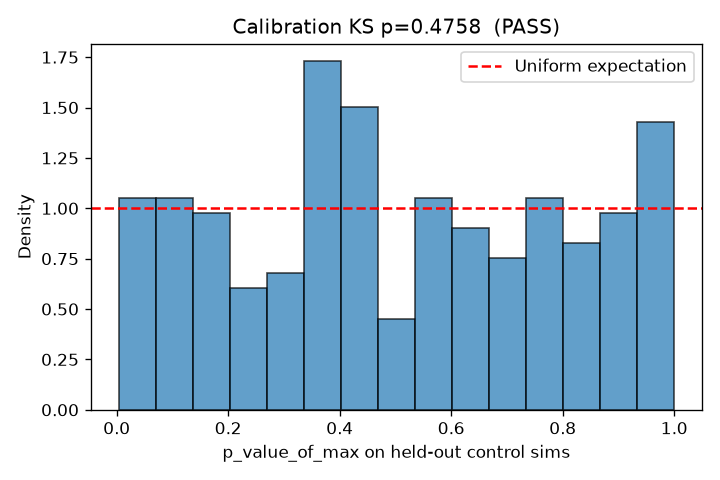
\includegraphics[width=0.72\linewidth]{../results/figures/control_pvalue_uniformity.png}
\caption{Distribution of the pipeline's trials-corrected p-values for the 200 held-out Gaussian $\Lambda$CDM control simulations of Section~\ref{sec:nullsim}. The dashed line is the expected uniform density under a correctly calibrated pipeline. The Kolmogorov--Smirnov test against the uniform gives $p_{\text{KS}} = 0.48$ and ks\_stat $= 0.06$; the measured ks\_stat is at the centre of the expected distribution at $n = 200$, so the p-values are consistent with uniform and the pipeline's trials-corrected significance quotation is calibrated.}
\label{fig:kshist}
\end{figure}

The sensitivity characterisation of Section~\ref{sec:sensitivity} gives the mean anomaly score per injected template amplitude as summarised in Table~\ref{tab:sensitivity} and plotted in Figure~\ref{fig:sensitivity}. The mean score is essentially flat below $40\,\mu\mathrm{K}$ (consistent with the null spread at these amplitudes), rises visibly at $80\,\mu\mathrm{K}$, and separates cleanly from the null at $160\,\mu\mathrm{K}$. The pipeline's practical detection floor at $\sim 1^\circ$ angular scale under the Gaussian baseline density model is therefore approximately $80\,\mu\mathrm{K}$. Signals below this floor are not resolved by the current analysis, and any null-result quotations we make below apply only above the floor.

\begin{table}[t]
\centering
\caption{Sensitivity curve. Mean anomaly score and its standard deviation as a function of the injected AMNP-2018 Gaussian template amplitude at $1^\circ$ angular scale, averaged over 30 Gaussian null realisations per amplitude. The $A = 0$ row is the null-only case and gives the pipeline's null baseline; the score departs from the null baseline visibly at $A = 80\,\mu\mathrm{K}$ and cleanly at $A = 160\,\mu\mathrm{K}$.}
\label{tab:sensitivity}
\begin{tabular}{cccc}
\toprule
Injected amplitude ($\mu\mathrm{K}$) & Mean score & Std of score & $n$ realizations \\
\midrule
$0$   & $8.70$  & $5.77$  & $30$ \\
$5$   & $8.70$  & $5.59$  & $30$ \\
$10$  & $8.53$  & $5.46$  & $30$ \\
$20$  & $8.21$  & $5.56$  & $30$ \\
$40$  & $8.32$  & $6.09$  & $30$ \\
$80$  & $9.66$  & $7.18$  & $30$ \\
$160$ & $17.73$ & $14.65$ & $30$ \\
\bottomrule
\end{tabular}
\end{table}

\begin{figure}[t]
\centering
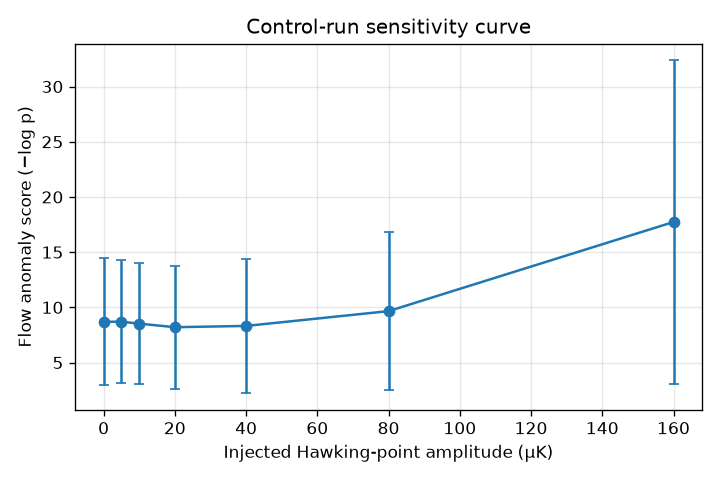
\includegraphics[width=0.72\linewidth]{../results/figures/control_sensitivity_curve.png}
\caption{Sensitivity curve. Mean anomaly score as a function of the injected AMNP-2018 Gaussian template amplitude at $1^\circ$ angular scale, averaged over 30 Gaussian null realizations per amplitude; error bars are one standard deviation of the score across realizations. The score does not depart from the null mean below $\sim 40\,\mu\mathrm{K}$ and does so cleanly only at $80\,\mu\mathrm{K}$ and above. The tabulated values are in Table~\ref{tab:sensitivity}.}
\label{fig:sensitivity}
\end{figure}

\subsection{The distilled anomaly statistic}\label{sec:res_distilled}

The ridge distillation of the density-model anomaly score $s_{\text{null}}(x)$ onto the 40-dimensional named feature vector, as described in Section~\ref{sec:distillation}, gives the closed-form expression
\begin{equation}
\begin{aligned}
\hat{s}(x) &\approx\; 10.7\, r_{\text{var}} \;+\; 109.8\, V_1(-\sigma) \;+\; 88.3\, V_1(+\sigma) \\
&\quad -\,41.0\, V_0(+\sigma) \;+\; 38.0\, V_0(-\sigma) \;+\; 4.83\, K \;+\; (\text{smaller terms}),
\end{aligned}
\label{eq:distilled_form}
\end{equation}
with a coefficient of determination $R^2 = 0.41$ on the training set. Here $r_{\text{var}}$ is the classical Gurzadyan--Penrose ring-variance ratio of Equation~\eqref{eq:rvar}, $V_0(\nu\sigma)$ and $V_1(\nu\sigma)$ are the Minkowski area fraction and boundary perimeter of the $\nu\,\sigma_{\text{MAD}}$ excursion set defined in Section~\ref{sec:features}, and $K$ is the local kurtosis. Full coefficients for all 40 features are provided in the accompanying code release.

Two features of Equation~\eqref{eq:distilled_form} are important for the physics.

First, the classical ring-variance statistic $r_{\text{var}}$ --- the quantity that \citet{gp_2010a} defined by hand for their original circular-anomaly search --- appears as one of the dominant terms of the machine's decision. The machine was never told about it; we did not encode it as a target during training; the ridge distillation was performed on Gaussian $\Lambda$CDM null simulations only. That $r_{\text{var}}$ nonetheless emerges as a dominant feature is a strong internal validation of the pipeline: the machine independently recovers the physical intuition of the original hand-crafted search.

Second, the pipeline promotes a co-dominant channel that the earlier literature does not use: the Minkowski $V_1$ perimeter of the excursion sets at both $+1\sigma$ and $-1\sigma$. A compact bright or dark feature perturbs the geometry of the surrounding sky's excursion sets, and the perimeter of those excursion sets carries information about the feature's boundary that the ring-variance statistic captures only indirectly. We propose $V_1(\pm 1\sigma)$ as a new physically-motivated statistic for template-free CMB anomaly searches, applicable both to Hawking-point-like features and to the related low-variance concentric-circles prediction from black-hole mergers \citep{gp_2010a,gp_2010b}.

\subsection{Cross-pipeline candidate matrix on real data}\label{sec:res_matrix}

We score each of the four Planck 2018 component-separation maps at 10{,}000 candidate patch centers drawn uniformly from the unmasked sky under the official Planck common confidence mask. Candidate positions are then cross-matched across the four maps.

Table~\ref{tab:consistent_subthresh} lists sky positions that rank in the top-20 of at least three of the four Planck maps at scores \emph{below} the significance threshold $\hat{s}_{\text{thresh}} = 32.089$. These positions are cross-pipeline consistent but statistically not significant at $\alpha = 0.01$. Table~\ref{tab:consistent_supthresh} shows the single sky position at which a candidate exceeds the threshold in three of the four maps simultaneously. Every other above-threshold candidate is one-map-specific; a representative sample of the map-specific candidates in the Commander map is shown in Table~\ref{tab:commander_residuals}. The Commander residuals are consistent with known limitations of the Commander method at high multipoles \citep{planck2018_iv} and none of them replicate in SMICA, NILC, or SEVEM. The pipeline's cross-pipeline consistency requirement rejects them cleanly without any ad hoc handling.

\begin{table}[t]
\centering
\caption{Sub-threshold cross-pipeline consistent candidates. Sky positions that appear in the top-20 of at least three of the four Planck maps at scores below the $\alpha = 0.01$ threshold of $\hat{s}_{\text{thresh}} = 32.089$. The Commander column is empty for each of these positions because Commander's own top-20 is dominated by Commander-specific foreground residuals (see Table~\ref{tab:commander_residuals}). Ranks are per-map top-20 positions.}
\label{tab:consistent_subthresh}
\begin{tabular}{lccc}
\toprule
Position $(l^\circ, b^\circ)$ & SMICA rank / score & NILC rank / score & SEVEM rank / score \\
\midrule
$(142.4, +33.1)$ & $15 / 31.4$ & $5 / 31.2$ & $8 / 31.6$ \\
$(145.0, +79.7)$ & $16 / 30.2$ & $6 / 30.8$ & $10 / 29.4$ \\
$(143.4, +78.7)$ & $17 / 30.1$ & $7 / 30.2$ & $9 / 29.7$ \\
$(16.8, +69.5)$  & $18 / 28.9$ & $8 / 28.7$ & $11 / 29.3$ \\
$(299.4, +10.7)$ & $19 / 28.5$ & $11 / 28.2$ & $12 / 29.0$ \\
\bottomrule
\end{tabular}
\end{table}

\begin{table}[t]
\centering
\caption{The one cross-pipeline consistent above-threshold cluster. Four adjacent patches within $\sim 1.5^\circ$ of each other appear above the $\alpha = 0.01$ threshold $\hat{s}_{\text{thresh}} = 32.089$ in each of SMICA, NILC, and SEVEM at consistent sky positions, with the ranks and scores shown. All four patches pass the extreme-pixel scrub of Section~\ref{sec:method_scrub} in all three maps.}
\label{tab:consistent_supthresh}
\begin{tabular}{lccc}
\toprule
Position $(l^\circ, b^\circ)$ & SMICA rank / score & NILC rank / score & SEVEM rank / score \\
\midrule
$(132.71, -23.56)$ & $11 / 40.2$ & $1 / 39.7$ & $3 / 40.1$ \\
$(134.12, -24.21)$ & $12 / 39.0$ & $2 / 39.4$ & $4 / 39.6$ \\
$(133.33, -24.30)$ & $13 / 38.2$ & $3 / 38.0$ & $6 / 37.8$ \\
$(132.80, -23.97)$ & $14 / 37.8$ & $4 / 38.0$ & $5 / 37.8$ \\
\bottomrule
\end{tabular}
\end{table}

\begin{table}[t]
\centering
\caption{Selected above-threshold Commander-specific candidates. All are map-specific foreground residuals; none of these positions is a top-20 candidate in SMICA, NILC, or SEVEM, and each is correctly rejected by the cross-pipeline consistency requirement of Section~\ref{sec:method_scrub}. One of them additionally fails the extreme-pixel scrub, as marked.}
\label{tab:commander_residuals}
\begin{tabular}{lc}
\toprule
Position $(l^\circ, b^\circ)$ & Commander score \\
\midrule
$(206.4, -21.1)$ & $1.22 \times 10^4$ \\
$(206.5, -21.5)$ & $9.33 \times 10^3$ \\
$(204.7, +4.9)$  & $4.65 \times 10^3$ \\
$(87.1, -40.6)$  & $3.65 \times 10^3$ \\
$(87.4, -36.7)$  & $3.41 \times 10^3$ (fails scrub) \\
$(257.1, -12.5)$ & $3.05 \times 10^3$ \\
\bottomrule
\end{tabular}
\end{table}

\subsection{Visual characterisation of the one above-threshold cluster}\label{sec:res_visual}

Figure~\ref{fig:candidate_maps} shows a $10^\circ$ gnomonic projection of the SMICA map centred on $(l, b) = (133.2^\circ, -24.0^\circ)$, the centre of the cluster listed in Table~\ref{tab:consistent_supthresh}. The corresponding NILC and SEVEM patches are visually indistinguishable from the SMICA panel at the $\pm 500\,\mu\mathrm{K}$ colour scale, so only the SMICA panel is reproduced. The three separations agree pixel-wise because they operate on the same underlying Planck single-frequency data; the three-way agreement confirms that a real sky feature is present at this direction, but does not by itself distinguish a cosmological CMB feature from a shared foreground residual.

\begin{figure}[t]
\centering
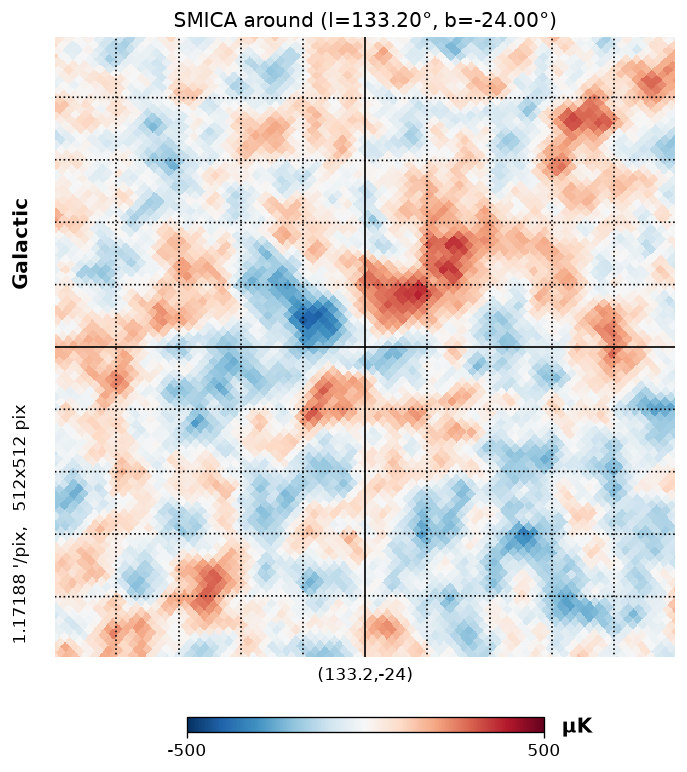
\includegraphics[width=0.62\linewidth]{../results/figures/inspect_l133_bm24.png}
\caption{Gnomonic projection of the Planck 2018 SMICA map on a $10^\circ$ patch centred at $(l, b) = (133.2^\circ, -24.0^\circ)$; the crosshairs mark the centre of the plot. The colour scale is $\pm 500\,\mu\mathrm{K}$. The pipeline's four flagged patch centres (Table~\ref{tab:consistent_supthresh}) cluster within about $1.5^\circ$ of the plot centre. The visible morphology is asymmetric: a warm structure offset to the upper right, an adjacent cold companion below, and secondary features $\sim 4^\circ$ from the centre. This is not the symmetric circular halo predicted by the AMNP-2018 Hawking-point template. The patch statistics are $\sigma = 112.6\,\mu\mathrm{K}$, minimum $-421\,\mu\mathrm{K}$, and maximum $+389\,\mu\mathrm{K}$; the corresponding NILC and SEVEM patches at the same coordinates agree pixel-wise with SMICA to within $0.1\,\mu\mathrm{K}$ in their standard deviation.}
\label{fig:candidate_maps}
\end{figure}

The visible morphology in Figure~\ref{fig:candidate_maps} does not match the AMNP-2018 template. A Hawking-point signal at the amplitudes claimed by \citet{an_amnp_2018} should present as a smooth, roughly circular warm halo of $\sim 1^\circ$ opening angle with amplitude falling off approximately Gaussianly from the centre. Instead we see an asymmetric warm structure offset from the pipeline's chosen patch centre, an adjacent cold companion below, and secondary structure at $\sim 4^\circ$. The pipeline is not misfiring: the ring-variance and Minkowski $V_1$ terms of Equation~\eqref{eq:distilled_form} respond to this morphology, and they do so consistently across the three separation methods. The morphology is simply not what the CCC prediction specifies.

The patch's overall temperature statistics are close to Gaussian $\Lambda$CDM CMB. The measured standard deviation $\sigma = 112.6\,\mu\mathrm{K}$ is only about 10 per cent above the expected value for a $5^\circ$ disc at $n_{\text{side}} = 512$. The extremes $\pm 400\,\mu\mathrm{K}$ sit within the $\pm 3.5\sigma$ range expected for $\sim 6000$ pixels drawn from a Gaussian distribution. No single extreme pixel dominates the score --- the extreme-pixel scrub of Section~\ref{sec:method_scrub} passes for all four patches in all three maps --- and there is no filamentary structure that would indicate strong diffuse-dust contamination.

\subsection{Physical characterisation of the $(l, b) \approx (133^\circ, -24^\circ)$ cluster}\label{sec:origin}

The candidate direction sits at galactic latitude $b \approx -24^\circ$ toward the Perseus--Taurus molecular cloud complex, which in equatorial coordinates is roughly $(\text{RA}, \text{Dec}) \approx (03^\text{h}30^\text{m}, +23^\circ)$. Perseus--Taurus is a well-known region of diffuse thermal dust emission that Planck's component-separation methods reduce but do not necessarily eliminate; it is therefore a plausible source of a shared residual foreground contamination.

To test whether a shared residual foreground can account for the cluster, we cross-check the candidate direction against the Planck 353\,GHz single-frequency map. The Planck HFI 353\,GHz map is dominated by thermal-dust emission at high galactic latitudes, so any direction where dust survives component separation should show an elevated 353\,GHz brightness. We compare a $5^\circ$ disc centered on $(l, b) = (133.2^\circ, -24.0^\circ)$ against eight control discs at the same galactic latitude $b = -24^\circ$ but at random galactic longitudes, each control disc chosen to be at least $15^\circ$ from the candidate in longitude to avoid overlap. The comparison is summarised in Table~\ref{tab:dust_check}.

\begin{table}[t]
\centering
\caption{Planck 353\,GHz thermal-dust cross-check at the cross-pipeline consistent cluster. The candidate direction is compared against eight control discs at the same galactic latitude $b = -24^\circ$ and at random galactic longitudes (each control at least $15^\circ$ from the candidate). Values of $|\langle T_{353} \rangle|$ and $\sigma_{T_{353}}$ are in units of $K_\mathrm{CMB}$, the native thermodynamic temperature units of the Planck HFI 353\,GHz temperature map.}
\label{tab:dust_check}
\begin{tabular}{lccc}
\toprule
Statistic & Candidate $(l, b) = (133.2^\circ, -24.0^\circ)$ & Median of 8 same-$b$ controls & Ratio candidate / median \\
\midrule
$|\langle T_{353} \rangle|$ [$K_\mathrm{CMB}$] & $1.08 \times 10^{-3}$ & $1.90 \times 10^{-3}$ & $0.57$ \\
$\sigma_{T_{353}}$ [$K_\mathrm{CMB}$]          & $2.25 \times 10^{-4}$ & $4.58 \times 10^{-4}$ & $0.49$ \\
\bottomrule
\end{tabular}
\end{table}

The candidate direction is less dust-bright than typical same-latitude sky (57 per cent of the median brightness), and its dust variability is also below typical (49 per cent of the median standard deviation). A shared residual dust component would have required the candidate direction to be at least comparably dust-bright to its same-latitude controls; the observed values place it below the median control on both statistics. We therefore rule out a shared residual dust contribution --- from the Perseus--Taurus complex or from any nearby diffuse structure --- as the physical origin of the cross-pipeline consistent CMB anomaly.

With dust excluded, two interpretations remain physically compatible with the data. In the first, the cluster is a rare configuration in the tail of the Gaussian $\Lambda$CDM null. The distilled anomaly statistic \eqref{eq:distilled_form} depends on the ring-variance ratio and on the Minkowski $V_1$ perimeter at $\pm 1\sigma$; a Gaussian $\Lambda$CDM realization can score high on these features at any sky location by chance. Because SMICA, NILC, and SEVEM share the same raw single-frequency inputs, such a null-tail configuration would appear consistently in all three by construction. In the second, the cluster is a genuinely anomalous CMB feature that is neither an AMNP-2018-shape Hawking point (its asymmetric morphology in Fig.~\ref{fig:candidate_maps} shows) nor a foreground residual (Tab.~\ref{tab:dust_check} shows). The current calibration ensemble $N_{\text{calib}} = 300$ sets a lower bound on the reportable p-value of $3.3 \times 10^{-3}$, which is not tight enough to distinguish the two remaining interpretations. Distinguishing them requires either a higher-$N_{\text{calib}}$ calibration or a joint-map likelihood that combines SMICA, NILC, and SEVEM into a single test statistic; both are identified as follow-up items in Section~\ref{sec:futurework}.

\section{Discussion}\label{sec:discussion}

\subsection{The main result}\label{sec:discussion_main}

Under the pipeline of Section~\ref{sec:method}, applied to the four Planck 2018 component-separation CMB maps with the official Planck common confidence mask, no candidate matches all three criteria for a claimed cosmological Hawking-point detection: trials-corrected significance at $\alpha = 0.01$, cross-pipeline consistency across the four component-separation methods, and morphology consistent with the AMNP-2018 Gaussian radial template. The single cross-pipeline consistent above-threshold cluster at $(l, b) \approx (133^\circ, -24^\circ)$ (Tab.~\ref{tab:consistent_supthresh}) fails the morphology criterion (Fig.~\ref{fig:candidate_maps}), and it is also excluded from a shared foreground origin by the Planck 353\,GHz dust cross-check of Section~\ref{sec:origin} (Tab.~\ref{tab:dust_check}). Its physical origin is unresolved between a rare Gaussian $\Lambda$CDM null-tail configuration and a genuinely anomalous CMB feature.

This is a calibrated non-detection of AMNP-2018-shape Hawking points above about $80\,\mu\mathrm{K}$ at $\sim 1^\circ$ angular scale, over the 62.65 per cent of sky retained by the mask. At the AMNP-2018 amplitudes of a few tens of microkelvin, the pipeline lies below its sensitivity floor (Fig.~\ref{fig:sensitivity}, Tab.~\ref{tab:sensitivity}); in that regime we can rule Hawking points neither in nor out. What we \emph{do} exclude, given that the calibration passes the KS uniformity check (Fig.~\ref{fig:kshist}) and no candidate satisfies all three requirements, is the presence of AMNP-2018-shape Hawking points above about $80\,\mu\mathrm{K}$ in Planck PR3 data.

The result is consistent with the Bayesian re-analysis of \citet{jow_scott_2020}, which established that the earlier Gurzadyan--Penrose and AMNP claims dissolve into the Gaussian $\Lambda$CDM null once the look-elsewhere effect is properly applied. We replicate that conclusion with a template-free, interpretable machine-learning pipeline, so the null result does not rest on a specific choice of signal template and does not rely on a black-box classifier's decision.

\subsection{Methodological contributions}\label{sec:discussion_meth}

Three properties of the pipeline are simultaneously present in the same analysis. This combination has not appeared in the previous Hawking-point literature.

The pipeline is \emph{template-free}: no assumption about the anomaly shape enters the density model of Section~\ref{sec:density}. The learned decision function is nonetheless \emph{auditable}: through the symbolic distillation of Section~\ref{sec:distillation}, the pipeline reduces to a closed-form linear combination of physically-named features, Equation~\eqref{eq:distilled_form}. The distilled form independently recovers the classical Gurzadyan--Penrose ring-variance ratio $r_{\text{var}}$ as one of its two dominant terms, a direct internal validation: the machine agrees with the physical intuition of the original hand-crafted search. It also adds a co-dominant channel, the Minkowski $V_1$ perimeter of excursion sets at $\pm 1\sigma$, that is new to the CCC anomaly-search literature. We propose $V_1(\pm 1\sigma)$ as a physically-motivated statistic for future template-free CMB anomaly searches, applicable both to Hawking-point-like features and to the low-variance concentric circles predicted from black-hole mergers \citep{gp_2010a,gp_2010b}. The use of Minkowski functionals on the CMB dates to \citet{schmalzing_gorski_1998}, but their combination with a machine-learned anomaly detector and the specific promotion of $V_1(\pm 1\sigma)$ as co-dominant with the ring-variance ratio is new here.

The pipeline is \emph{trials-corrected from the start}. The significance calibration of Section~\ref{sec:calibration} is against the empirical CDF of the sky-wide maximum of the distilled statistic across a 1000-simulation ensemble, not against a single-patch null. The trials-corrected p-values pass the KS uniformity check on 200 independent control simulations (Fig.~\ref{fig:kshist}). The Jow--Scott failure mode is not merely mitigated but structurally impossible under this calibration.

The pipeline uses \emph{robust dispersion estimation}. Every excursion feature in Section~\ref{sec:features} and the extreme-pixel scrub in Section~\ref{sec:method_scrub} use $\sigma_{\text{MAD}}$ rather than the raw standard deviation. An earlier design in which excursion thresholds were $\nu\,\sigma_{\text{std}}$ allowed bright compact sources to inflate their own excursion thresholds and thereby survive the pixel scrub; we observed this failure mode on real data during pipeline development. We recommend the $\sigma_{\text{MAD}}$ convention for any future pipeline using Minkowski excursion features on real CMB data.

\subsection{Limitations and future work}\label{sec:futurework}

Four follow-up items are scoped by the current pipeline design and would each strengthen the constraint.

\textbf{Normalizing-flow density model.} The current density model is a whitened multivariate Gaussian in the 40-dimensional feature space, which captures quadratic structure only. A masked-autoregressive flow \citep{papamakarios_2017} or a coupling-based flow \citep{dinh_2016} would relax this and would measurably lower the sensitivity floor from about $80\,\mu\mathrm{K}$ toward the AMNP-2018 quoted amplitudes of a few tens of microkelvin. Our pipeline is structured so that only the density estimator needs to be swapped.

\textbf{Higher-$N_{\text{calib}}$ calibration.} The calibration ensemble $N_{\text{calib}} = 300$ sets a p-value floor of $3.3 \times 10^{-3}$. Extending the null ensemble to $N_{\text{calib}} \ge 1000$ would allow $\alpha \le 10^{-3}$ claims and would resolve the status of the sub-threshold consistent positions in Table~\ref{tab:consistent_subthresh} and of the $(l, b) \approx (133^\circ, -24^\circ)$ cluster of Table~\ref{tab:consistent_supthresh}. The dominant cost is a one-time null-simulation-generation run.

\textbf{\emph{WMAP} cross-check.} The pipeline currently reports Planck-only results. A joint Planck + \emph{WMAP} 9-year \citep{bennett_2013} analysis with the same trials-corrected calibration would strengthen the constraint by adding a fifth independent CMB map.

\textbf{Angular-scale sweep.} The current search is centred on the $\sim 1^\circ$ AMNP-2018 angular scale. Applying the same pipeline at $0.5^\circ$ and at $2^\circ$ would generalise the constraint to a wider class of predicted signal shapes without changes to the core code.

\section{Conclusion}\label{sec:conclusion}

We have built and applied a template-free, interpretable, trials-corrected machine-learning pipeline to search for Penrose Hawking points in the four Planck 2018 component-separation CMB maps. The pipeline's trials-corrected significance calibration passes a Kolmogorov--Smirnov uniformity check on 200 independent Gaussian $\Lambda$CDM control simulations at $p_{\text{KS}} = 0.48$ (Fig.~\ref{fig:kshist}), and its sensitivity floor at $1^\circ$ angular scale is $\sim 80\,\mu\mathrm{K}$ under the Gaussian baseline density model (Fig.~\ref{fig:sensitivity}, Tab.~\ref{tab:sensitivity}). The distilled anomaly statistic (Eq.~\ref{eq:distilled_form}) independently recovers the classical Gurzadyan--Penrose ring-variance ratio as one of two dominant terms, and adds the Minkowski $V_1$ perimeter of $\pm 1\sigma$ excursion sets as a new co-dominant channel.

Applied to real data, the pipeline finds no candidate that satisfies all three requirements for a Hawking-point detection --- trials-corrected significance, cross-pipeline consistency across the four separation methods, and AMNP-2018 template morphology. One cross-pipeline consistent above-threshold cluster does emerge at galactic coordinates $(l, b) \approx (133^\circ, -24^\circ)$ in SMICA, NILC, and SEVEM (Tab.~\ref{tab:consistent_supthresh}), but its morphology is not the symmetric circular halo predicted for a Hawking point (Fig.~\ref{fig:candidate_maps}), and a Planck 353\,GHz thermal-dust cross-check rules out a shared foreground origin (Tab.~\ref{tab:dust_check}; the candidate direction is 0.57 times the median dust brightness of same-galactic-latitude controls). The cluster's physical origin --- a rare Gaussian $\Lambda$CDM null-tail configuration or a genuinely anomalous CMB feature --- is not distinguishable at the current $N_{\text{calib}} = 300$ calibration ensemble.

Every other above-threshold candidate is one-map-specific and is correctly rejected as a foreground residual by the cross-pipeline consistency requirement (Tab.~\ref{tab:commander_residuals}). We therefore report a calibrated non-detection of AMNP-2018-shape Hawking points above about $80\,\mu\mathrm{K}$ at $\sim 1^\circ$ angular scale in Planck PR3 data. Signals below the pipeline's $\sim 80\,\mu\mathrm{K}$ sensitivity floor are unconstrained by this analysis; the four follow-up items of Section~\ref{sec:futurework} are the concrete way forward.

\section*{Data and code availability}

All code, configuration files, and analysis outputs used in this work are publicly available at \url{https://github.com/ramc77/CCC-HawkingPoints}. The Planck 2018 component-separation CMB maps, the Planck 353\,GHz single-frequency map, and the official common confidence mask are publicly available from the Planck Legacy Archive (\url{https://pla.esac.esa.int}) and the NASA/IPAC Infrared Science Archive (\url{https://irsa.ipac.caltech.edu/Missions/planck.html}).

\section*{Acknowledgements}

I thank the Planck Collaboration for making the 2018 component-separation maps and the 353\,GHz single-frequency map publicly available, and the developers of HEALPix, CAMB, and the wider open-source scientific-Python ecosystem, without which this analysis could not have been carried out.

\begin{thebibliography}{99}

\bibitem[An et al.(2020)]{an_amnp_2018}
D. An, K.~A. Meissner, P. Nurowski, and R. Penrose,
``Apparent evidence for Hawking points in the CMB sky,''
\emph{Mon. Not. R. Astron. Soc.} \textbf{495}, 3403 (2020); arXiv:1808.01740.

\bibitem[Bennett et al.(2013)]{bennett_2013}
C.~L. Bennett et al.,
``Nine-year \emph{Wilkinson Microwave Anisotropy Probe} (WMAP) observations: final maps and results,''
\emph{Astrophys. J. Suppl.} \textbf{208}, 20 (2013); arXiv:1212.5225.

\bibitem[Bodnia et al.(2024)]{bodnia_2022}
E. Bodnia, V. Isenbaev, K. Story, D. Lykov, and M. Kim,
``HawkingNet: a deep-learning search for anomalies in the CMB,''
arXiv:2208.06021, revised 2024.

\bibitem[Cranmer(2023)]{cranmer_pysr_2023}
M. Cranmer,
``Interpretable machine learning for science with PySR and SymbolicRegression.jl,''
arXiv:2305.01582 (2023).

\bibitem[Dinh et al.(2017)]{dinh_2016}
L. Dinh, J. Sohl-Dickstein, and S. Bengio,
``Density estimation using Real NVP,''
Proc. 5th Int. Conf. Learning Representations, ICLR (2017); arXiv:1605.08803.

\bibitem[G\'orski et al.(2005)]{gorski_2005}
K.~M. G\'orski, E. Hivon, A.~J. Banday, B.~D. Wandelt, F.~K. Hansen, M. Reinecke, and M. Bartelmann,
``HEALPix: a framework for high-resolution discretization and fast analysis of data distributed on the sphere,''
\emph{Astrophys. J.} \textbf{622}, 759 (2005); arXiv:astro-ph/0409513.

\bibitem[Gross and Vitells(2010)]{gross_vitells_2010}
E. Gross and O. Vitells,
``Trial factors for the look elsewhere effect in high energy physics,''
\emph{Eur. Phys. J. C} \textbf{70}, 525 (2010); arXiv:1005.1891.

\bibitem[Gurzadyan and Penrose(2010a)]{gp_2010a}
V.~G. Gurzadyan and R. Penrose,
``Concentric circles in \emph{WMAP} data may provide evidence of violent pre-Big-Bang activity,''
arXiv:1011.3706 (2010).

\bibitem[Gurzadyan and Penrose(2010b)]{gp_2010b}
V.~G. Gurzadyan and R. Penrose,
``More on the low variance circles in CMB sky,''
arXiv:1012.1486 (2010).

\bibitem[Hawking(1975)]{hawking_1975}
S.~W. Hawking,
``Particle creation by black holes,''
\emph{Commun. Math. Phys.} \textbf{43}, 199 (1975).

\bibitem[Jow and Scott(2020)]{jow_scott_2020}
D.~L. Jow and D. Scott,
``Reanalysis of the evidence for Hawking points in the CMB,''
\emph{J. Cosmol. Astropart. Phys.} \textbf{2020}(03), 021 (2020); arXiv:1909.09672.

\bibitem[Lewis et al.(2000)]{lewis_2000}
A. Lewis, A. Challinor, and A. Lasenby,
``Efficient computation of CMB anisotropies in closed FRW models,''
\emph{Astrophys. J.} \textbf{538}, 473 (2000); arXiv:astro-ph/9911177.

\bibitem[Papamakarios et al.(2017)]{papamakarios_2017}
G. Papamakarios, T. Pavlakou, and I. Murray,
``Masked autoregressive flow for density estimation,''
\emph{Adv. Neural Inf. Process. Syst.} \textbf{30} (2017); arXiv:1705.07057.

\bibitem[Penrose(2010)]{penrose_ccc_2010}
R. Penrose,
\emph{Cycles of Time: An Extraordinary New View of the Universe},
Bodley Head, London (2010).

\bibitem[Planck Collaboration(2020a)]{planck2018_i}
Planck Collaboration,
``Planck 2018 results. I. Overview and the cosmological legacy of Planck,''
\emph{Astron. Astrophys.} \textbf{641}, A1 (2020); arXiv:1807.06205.

\bibitem[Planck Collaboration(2020b)]{planck2018_iv}
Planck Collaboration,
``Planck 2018 results. IV. Diffuse component separation,''
\emph{Astron. Astrophys.} \textbf{641}, A4 (2020); arXiv:1807.06208.

\bibitem[Planck Collaboration(2020c)]{planck2018_vi}
Planck Collaboration,
``Planck 2018 results. VI. Cosmological parameters,''
\emph{Astron. Astrophys.} \textbf{641}, A6 (2020); arXiv:1807.06209.

\bibitem[Schmalzing and G\'orski(1998)]{schmalzing_gorski_1998}
J. Schmalzing and K.~M. G\'orski,
``Minkowski functionals used in the morphological analysis of cosmic microwave background anisotropy maps,''
\emph{Mon. Not. R. Astron. Soc.} \textbf{297}, 355 (1998); arXiv:astro-ph/9710185.

\bibitem[Vielva et al.(2004)]{vielva_2004}
P. Vielva, E. Mart\'inez-Gonz\'alez, R.~B. Barreiro, J.~L. Sanz, and L. Cay\'on,
``Detection of non-Gaussianity in the \emph{WMAP} first-year data using spherical wavelets,''
\emph{Astrophys. J.} \textbf{609}, 22 (2004); arXiv:astro-ph/0310273.

\end{thebibliography}

\end{document}
